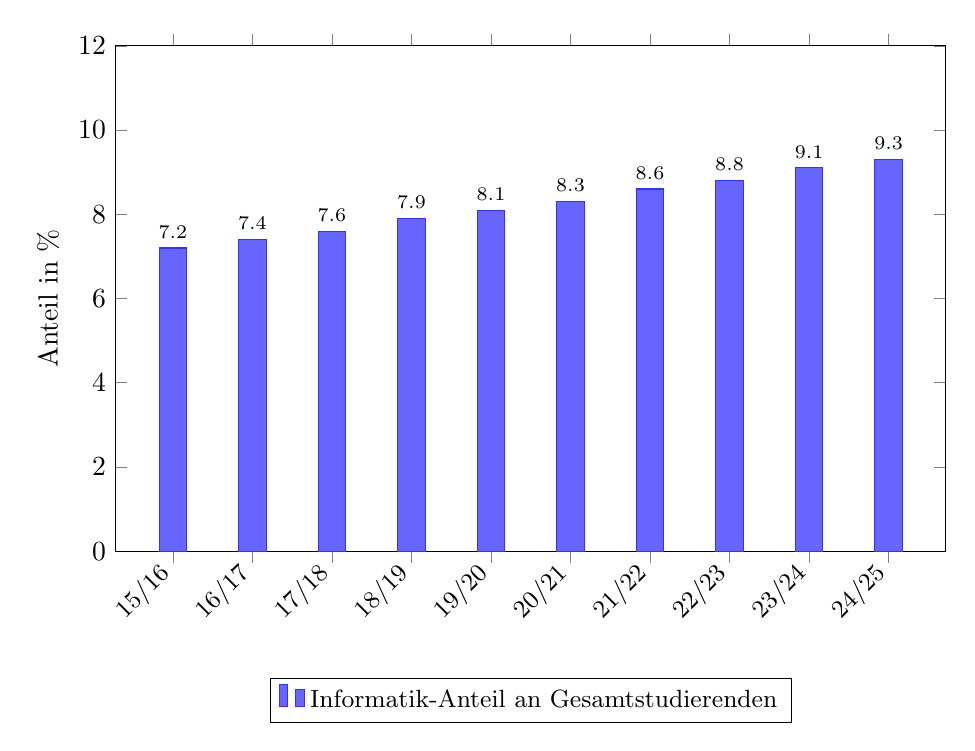
\begin{tikzpicture}
\begin{axis}[
    ybar,
    width=\textwidth,
    height=8cm,
    bar width=10pt,
    ylabel={Anteil in \%},
    symbolic x coords={15/16, 16/17, 17/18, 18/19, 19/20, 20/21, 21/22, 22/23, 23/24, 24/25},
    xtick=data,
    x tick label style={rotate=45, anchor=east, font=\small},
    ymin=0,
    ymax=12,
    ytick={0,2,4,6,8,10,12},
    nodes near coords,
    nodes near coords align={vertical},
    every node near coord/.append style={font=\scriptsize, /pgf/number format/fixed, /pgf/number format/precision=1},
    enlarge x limits=0.08,
    legend style={at={(0.5,-0.25)}, anchor=north, legend columns=-1, font=\small},
]
% Anteil Informatik (Studienbereich) an Gesamtstudierenden
% Quellen: Destatis (WS 22/23--24/25), CHE Arbeitspapier 200 (WS 16/17),
%          CHE DatenCHECK 3/2022 (WS 21/22); Zwischenwerte interpoliert
% WS 15/16: ~198.000 / 2.757.799 = 7.2%
% WS 16/17: 207.356 / 2.807.010 = 7.4%  (CHE)
% WS 17/18: ~217.000 / 2.844.978 = 7.6%
% WS 18/19: ~226.000 / 2.868.222 = 7.9%
% WS 19/20: ~235.000 / 2.897.297 = 8.1%
% WS 20/21: ~244.000 / 2.948.695 = 8.3%
% WS 21/22: 253.540 / 2.946.100 = 8.6%  (CHE)
% WS 22/23: 257.164 / 2.915.700 = 8.8%  (Destatis)
% WS 23/24: 260.078 / 2.868.300 = 9.1%  (Destatis)
% WS 24/25: 267.249 / 2.871.600 = 9.3%  (Destatis)
\addplot[fill=blue!60, draw=blue!80] coordinates {
    (15/16, 7.2)
    (16/17, 7.4)
    (17/18, 7.6)
    (18/19, 7.9)
    (19/20, 8.1)
    (20/21, 8.3)
    (21/22, 8.6)
    (22/23, 8.8)
    (23/24, 9.1)
    (24/25, 9.3)
};
\legend{Informatik-Anteil an Gesamtstudierenden}
\end{axis}
\end{tikzpicture}
